\section{Verteiltes TensorFlow}
Nachdem im vorherigen Kapitel einen kleiner Überblick über TensorFlow gegeben wurde, soll jetzt die Verteilung einer TensorFlow Umgebung auf mehrere Instanzen näher betrachtet werden. Dieses Kapitel stellt nötiges Wissen bereit, dass im nächsten Kapitel im Rahmen eines Tutorials zur Einrichtung einer verteilten TensorFlow Umgebung eingesetzt wird. 

\subsection{Architektur}
Im folgenden wird die Architektur einer verteilten TensorFlow Umgebung genauer beschrieben. Dabei wird zwischen dem Paramter Server und Arbeiter unterschieden.

\subsubsection{Parameterserver}
Der Parameterserver verwaltet das aktuelle Model mit seinen Gewichtungen und Variablen und verteilt es an die Arbeiter. Falls durch mehrere Arbeiter zu viel Ein-/Ausgabe Anfragen an den Parameterserver erzeugt werden, können mehrere Parameterserver eingesetzt werden, um die Last zu verteilen. Mehreren Parameterserver synchronisieren das Model untereinander. Abbildung \ref{fig:architektur-servemodel} zeigt, wie das Verteilen des Models an die Arbeiter aussehen kann. 

\begin{figure}[h!]
	\centering
	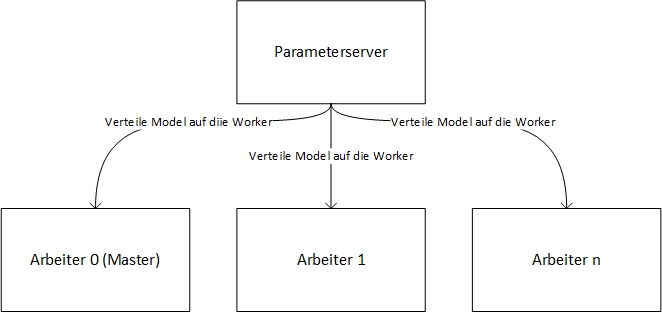
\includegraphics[width=0.9\linewidth]{Pictures/Architektur-ServeModel}
	\caption[Verteilen des Models auf die Arbeiter]{Verteilen des Models auf die Arbeiter}
	\label{fig:architektur-servemodel}
\end{figure}

\subsubsection{Arbeiter}
Arbeiter führen ressourcenintensive Berechnung durch zur Optimierung des vom Parameterserver bereitgestellten Models. Nach der Optimierung sendet der Arbeiter das neue Model mit seinen Gewichtungen und Variablen zum Parameterserver. Desto mehr Arbeiter eingesetzt werden, desto schneller und effizienter kann ein Model trainiert werden. Abbildung \ref{fig:architektur-updatemodel} zeigt, wie die Berechnung des Models und die Aktualisierung des Models auf dem Parameterserver aussehen kann. Der Master Arbeiter koordiniert die Trainingsvorgänge und kümmert sich um die Initialisierung des Modells, Zählen der Anzahl der ausgeführten Trainingsschritte, Speichern und Wiederherstellen von Modellkontrollpunkten.

\begin{figure}[h!]
	\centering
	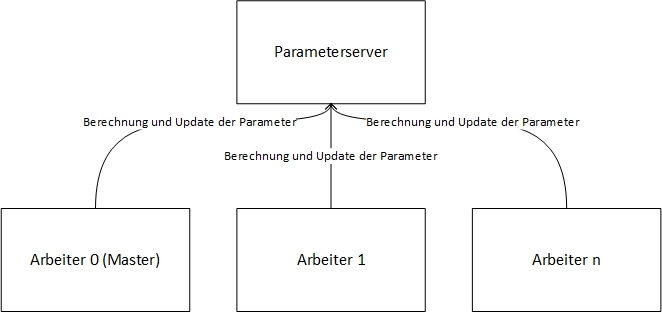
\includegraphics[width=0.9\linewidth]{Pictures/Architektur-UpdateModel}
	\caption[Berechnung des Models auf Arbeiter + Updaten der Variablen auf dem Parameterserver]{Berechnung des Models auf Arbeiter + Updaten der Variablen auf dem Parameterserver}
	\label{fig:architektur-servemodel}
\end{figure}

\subsection{Datenparallelität}
Es gibt zwei verschiedene Möglichkeiten für Datenparallelität:
\subsubsection{Synchron}
Die Arbeiter lesen gleichzeitig das Model vom Parameterserver und berechnen mit diesem ihre Trainingsoperationen und warten, bis die anderen Arbeiter fertig sind. Dann werden die Ergebnisse gemittelt und eine Aktualisierung des Models wird an den Parameterserver gesendet. Somit hat zu jedem Zeitpunkt jeder Arbeiter das gleiche Model.

\subsubsection{Asynchron}
Die Arbeiter lesen asynchron von den Parameterserver, berechnen ihre Trainingsoperation und senden asynchrone Aktualisierungen an den Parameterserver. Zu jedem Zeitpunkt könnten zwei verschiedene Arbeiter unterschiedliche Werte für ihr Model besitzen.

\subsection{Weitere Möglichkeiten}
Bisher wurde die einfachste Methode beschrieben, wie ein verteilte TensorFlow Umgebung eingerichtet werden kann. 




